\documentclass[crop,tikz,convert={outext=.svg,command=\unexpanded{pdf2svg \infile\space\outfile}},multi=false]{standalone}[2012/04/13]
\usepackage{tikz}
\usepackage{pgfplots}
\usetikzlibrary{arrows,shapes,positioning}
\begin{document}
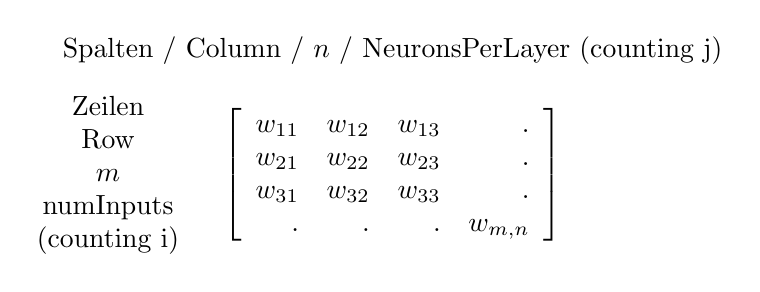
\begin{tikzpicture}[->,>=latex',shorten >=1pt,auto,node distance=0.3cm,
                    thick]
\tikzstyle{komp}=[rectangle,thick,draw=black,minimum size=10mm]
\tikzstyle{mot}=[circle,thick,draw=black,minimum size=5mm]
\node[align=center] (matrix) {$\left[ \begin{array}{rrrr}
   w_{11} & w_{12} & w_{13} & .
\\ w_{21} & w_{22} & w_{23} & .
\\ w_{31} & w_{32} & w_{33} & .
\\ . & . & . & w_{m,n}
\end{array} \right]$};
\node[align=center](zeilen)[left=of matrix] {Zeilen\\ Row \\ $m$ \\ numInputs \\ (counting i)};
\node[align=center](zeilen)[above=of matrix] {Spalten / Column /  $n$ / NeuronsPerLayer (counting j)};
\end{tikzpicture}
\end{document}